%----------------------------------------------------------------------------
%----------------------------------------------------------------------------
%				    	SETUP
%----------------------------------------------------------------------------
%----------------------------------------------------------------------------

\documentclass[11pt]{article}

%----------------------------------------------------------------------------
%			  	   PACKAGES
%----------------------------------------------------------------------------

%%%%%%%%%%%%%%%%%%%%%%%
% 	  Packages
%%%%%%%%%%%%%%%%%%%%%%%

%% Fonts and Symbols
%% --------------------------
\usepackage{
	amsmath,			% math operators
	amssymb,			% math symbols
	courier,			% better tt font for listings
	soul,				% strike through with \st{}
	url,				% embed urls in text
	xcolor,				% color!
%	xfrac,				% fancy fractions
}

% preserve default font for URLs
\renewcommand*{\UrlFont}{\rmfamily}		

%% Graphics
%% --------------------
\usepackage{
	graphicx,			% allows insertion of images
	subfigure,			% allows subfigures (a), (b), etc.
}				
\graphicspath{ {graphics/} }	% (graphicx) relative path to graphics folder				

%% Tables
%% --------------------------
\usepackage{
	booktabs,			% better tables, discourages vertical rulings
	multicol,			% allow multi columns
}

%% Layout Alteration
%% --------------------------
\usepackage{			
%	caption,			% line breaks in captions with \\
%	changepage,			% change margins for PARTS of pages with (adjustwidth)
	geometry,			% change the margins for specific PAGES
	parskip,			% disable indents
	rotating,			% sideways figures
	setspace,			% single, double spacing
}
\geometry{				% specify page size options for (geometry)
	a4paper, 			% paper size
	hmargin=1in,		% horizontal margins
	vmargin=1in,		% vertical margins
}	


%% Units
%% --------------------------
\usepackage{
	siunitx,			% has S (decimal align) column type
}
\sisetup{input-symbols = {()},  % do not treat "(" and ")" in any special way
	group-digits  = false, 	% no grouping of digits
%	load-configurations = abbreviations,
%	per-mode = symbol,
}

%% Misc
%% --------------------------
\usepackage{
	enumitem,			% better control of enumerations, descriptions, etc
%	listings,			% source code import and display
	todonotes,			% gives \todo[inline]{stuff} and \missingfigure{description}
}

%% References
%% --------------------------
\usepackage[backend=biber,style=ieee]{biblatex}
\addbibresource{ELEC340_Lab_04.bib}

%----------------------------------------------------------------------------
%		     MACROS AND COMMANDS
%----------------------------------------------------------------------------

% Defines a new command for the horizontal lines, change thickness here
\newcommand{\HRule}{\rule{\linewidth}{0.5mm}} 

% override S column type with centered text column
\newcommand{\textcol}[1]{\multicolumn{1}{c}{#1}}

% awkward capitalization
\newcommand{\mefisto}{MEFiSTo}

% bold vectors
\newcommand{\vect}[1]{\ensuremath{\mathbf{#1}}}

% activate to override bold vectors to arrows
%\renewcommand{\vect}[1]{\vec{#1}}​

% phasors!
\newcommand{\phasor}[1]{\tilde{\mathbf{#1}}}

% unit vectors
\newcommand{\unitvec}[1]{\hat{\mathbf{#1}}}

%----------------------------------------------------------------------------
%----------------------------------------------------------------------------
%				   DOCUMENT
%----------------------------------------------------------------------------
%----------------------------------------------------------------------------

\begin{document}

\begin{titlepage}

\center
 
% Header
\textsc{\LARGE University of Victoria}\\[1cm] 	% Name of your university/college
\textsc{\Large ELEC 340}\\[0.5cm] 			% Major heading such as course name
\textsc{\large Applied Electromagnetics and Photonics}\\[0.5cm] 		% Minor heading such as course title


% Lab Title
\HRule \\[0.4cm]
{\huge \bfseries Lab 1 - Time-Varying Electromagnetic Fields}\\[0.2cm] % Title of your document
\HRule \\[1.5cm]
 
 
%Lab Instructor Details
\begin{minipage}{0.7\textwidth}
\begin{flushleft} 

\large\emph{Instructor:} \\
Dr. Poman \textsc{So} \\
\vspace{12 pt}
% I don't know the name of our TA :(
%\emph{Teaching Assistant:} \\ 
%Grace \textsc{Hui}

\end{flushleft}
\end{minipage}
~
\begin{minipage}{0.1\textwidth}
\begin{flushright} \large

\vspace{12 pt}

\end{flushright}
\end{minipage}\\[2cm]


% Lab members
\Large A.K. \textsc{Blanken}
\large V00809798 \\
\Large T. \textsc{Stephen}
\large V00812021	\\
A01 - B03\\[1.5cm] 


{\large 3 February, 2016}\\ % Date

\begin{figure}[b]
	\centering
	\includegraphics[scale=0.3]{UVic_logo}
\end{figure}

\end{titlepage}


\doublespacing
\section{Objective}\label{sec:objective}
This experiment will use a \mefisto{} simulation to investigate the propagation of an electromagnetic wave through a waveguide.
The results of the simulation will validate the Helmholtz equation and provide insight into the propagation properties of plane waves.

\section{Introduction}\label{sec:intro}
This experiment used \mefisto{} to explore the refraction of electromagnetic waves at oblique incidence.
Waves at \SI{45}{\degree} incidence were explored with different permittivity transitions. 

A Brewster angle interface was constructed so that an electromagnetic wave could strike at oblique incidence but not experience reflection.
This occurs when the incidence is
\begin{equation}\label{eqn:brewster}
	\tan\theta_B = \sqrt{{\epsilon_2 \over \epsilon_1}}.
\end{equation}
The behavior of electromagnetic waves in a cavity was examined next.
An impulse function was used to determine the resonant frequencies of a cavity with $a = \SI{30}{mm}$ and $b = \SI{20}{\milli\meter}$.
These resonant frequencies determine which transmission modes will be permitted.

Lastly, we downloaded a pre-built \mefisto{} waveguide and altered the mode and generating frequency to create new transmission modes for the same waveguide.

\section{Discussion}\label{sec:discussion}
\paragraph{Task 4} \textit{Compare the phase velocity to what you found in Section \ref{sec:upw}.}

By recording the distance traveled by a wave peak in one step of the animation, we found that:
\begin{equation*}
	u_{ph} = {\Delta x \over \Delta t} = {\SI{0.5}{\milli\meter} \over \SI{0.166}{\pico\second}} = \SI{3.01E8}{\meter\per\second}.
\end{equation*}
We found that $\lambda = \SI{20}{\milli\meter}$ in Section \ref{sec:upw} which implies that $u_{ph} = c_0$. The discrepancy between the two numbers is likely the result of a rounding error in \mefisto.

\paragraph{Task 7} \textit{Reduce the plate spacing to 4 mm and increase the width to 14 mm in the environment used for Section \ref{sec:non-ideal}.
Does the far field in the $xy$ and $yz$ planes behave like a uniform plane wave?}

Narrowing the gap between the electric field boundaries and widening them creates the propagation patterns shown in Fig. \ref{fig:narrow}.

\begin{figure}[htpb]
	\centering
	\subfigure[]
	{
		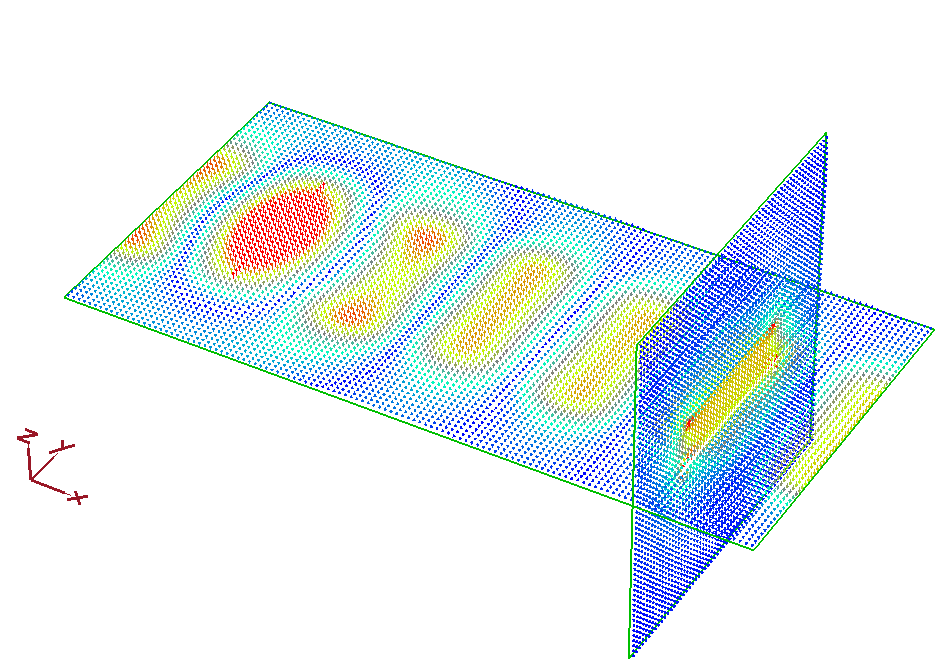
\includegraphics[width=0.575\linewidth]{graphics/Task2-3d-narrowplate}
		\label{fig:3d-narrow}
	}
	\subfigure[$yz$-orientation]
	{
		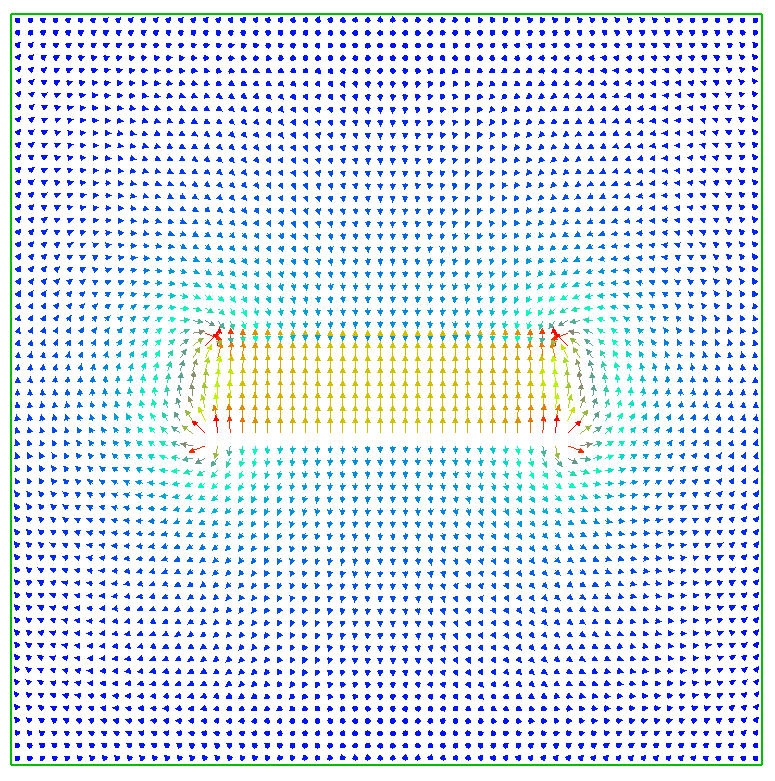
\includegraphics[width=0.375\linewidth]{graphics/Task2-yz-narrowplate}
		\label{fig:yz-narrow}
	}
	\caption{Propagation in a non-ideal, narrow parallel plate}
	\label{fig:narrow}
\end{figure}

The magnitude of the waves in Fig. \ref{fig:narrow}\subref{fig:3d-narrow} is greater than those in Fig. \ref{fig:non-ideal}\subref{fig:3d} and the groups have a much shorter and wider region of similar magnitude.
Fig. \ref{fig:narrow}\subref{fig:yz-narrow} confirms that both the direction and magnitude of the wave are similar far from the source.
Changing the electric field arrangement to make the separation smaller and boundaries wider has restored the plane wave behavior for the region between the boundaries.

\paragraph{Task 8} \textit{Determine $\alpha$ and $\beta$ for the waveguide with dielectric from Section \ref{sec:dielectric}.}

The lab manual suggests using Fig. \ref{fig:Task3-mesh} to determine the attenuation of the wave with equations \eqref{eqn:alpha} and \eqref{eqn:beta}.

\begin{figure}[tbph]
	\centering
	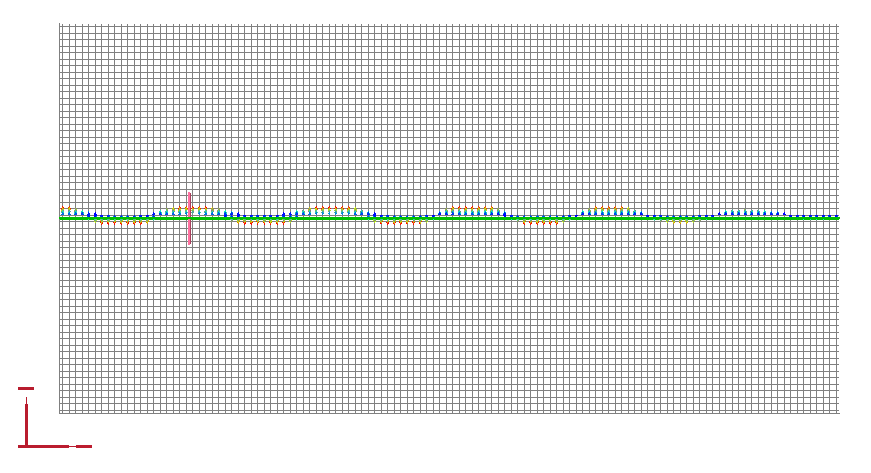
\includegraphics[width=0.7\linewidth]{graphics/Task3-mesh}
	\caption{$xz$ view of Fig. \ref{fig:Task3-3d-animation}}
	\label{fig:Task3-mesh}
\end{figure}
\begin{align}
	\alpha &= { \ln \left( { E_z(x_1) \over E_z(x_2) } \right) \over m \Delta x } \label{eqn:alpha} \\
	\beta &= { 2 \pi \over \lambda } \label{eqn:beta}
\end{align}
This method poses a problem since the magnitude of the electric field is not displayed on the graph.
Determining the ratio of two points is extremely imprecise.

In order to obtain more accurate measurements of $E_z$, a second probe was added to the animation \SI{5}{\milli\meter} closer to the source than the probe in Fig. \ref{fig:waveguide}.
The $E_z$ response at both probes is shown in Fig. \ref{fig:Task3-probes}. 

\begin{figure}[tbph]
	\centering
	\subfigure[35 mm]
	{
		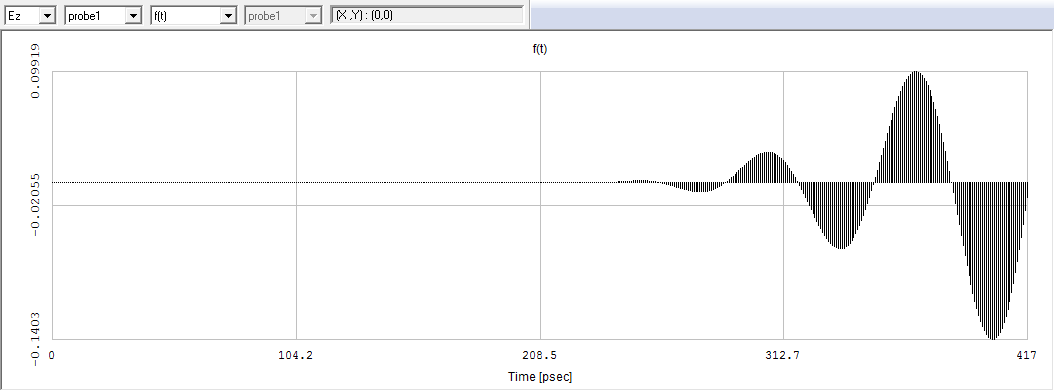
\includegraphics[width=0.95\linewidth]{graphics/35mm}
	}
	\subfigure[40 mm]
	{
		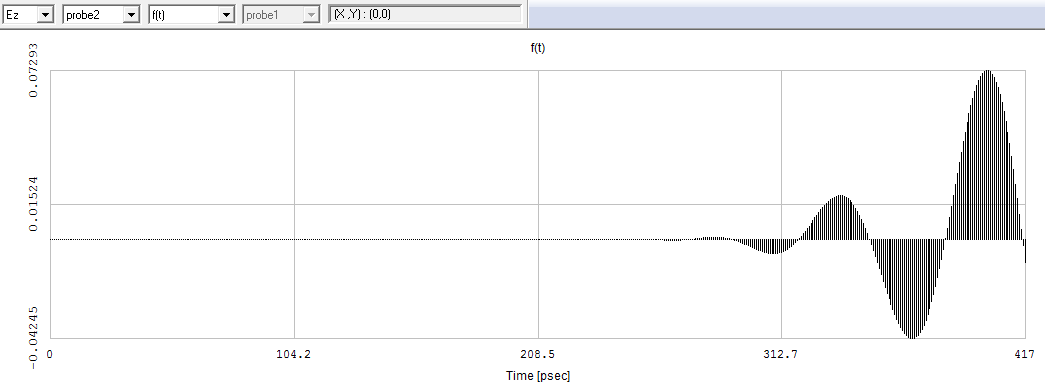
\includegraphics[width=0.95\linewidth]{graphics/40mm}
	}
	\caption{$E_z$ response at different distances from source}
	\label{fig:Task3-probes}
\end{figure}

Using the peak positive value for both probes with \eqref{eqn:alpha} gives:
\begin{equation*}
	\alpha = { \ln \left( { \SI{0.09919}{\volt\per\meter} \over \SI{0.07293}{\volt\per\meter} } \right) \over \SI{5}{\milli\meter}} = \SI{55.9}{\neper\per\meter}.
\end{equation*}
Using $\lambda = \SI{10}{mm}$ in \eqref{eqn:beta}:
\begin{equation*}
	\beta = {2 \pi \over \lambda} = \SI{628.31}{\radian\per\meter}.
\end{equation*}

\paragraph{Task 9} \textit{Compare the results of Task 8 to the theoretical values.}

The attenuation and phase constants are:
\begin{align*}
	\alpha &= { \omega \sqrt{\mu \epsilon} \over \sqrt{2} } \sqrt{\sqrt{1 + \left( {\sigma \over \omega \epsilon} \right)^2} - 1} \\
	&= { \omega \sqrt{\epsilon_r} \over c_0 \sqrt{2} } \sqrt{\sqrt{1 + \left( {\sigma \over \omega \epsilon_0 \epsilon_r} \right)^2} - 1} \\
	&= { 2 \pi \cdot \SI{15}{\giga\hertz} \cdot \sqrt{4} \over c_0 \sqrt{2} } \sqrt{\sqrt{1 + \left( {0.5 \over 2 \pi \cdot \SI{15}{\giga\hertz} \cdot \epsilon_0 \cdot 4} \right)^2} - 1} \\
	&= \SI{46.96}{\neper\per\meter}
\end{align*}
\begin{align*}
	\beta &= { \omega \sqrt{\mu \epsilon} \over \sqrt{2} } \sqrt{\sqrt{1 + \left( {\sigma \over \omega \epsilon} \right)^2} + 1} \\
	&= \SI{630.50}{\radian\per\meter}
\end{align*}

The numbers agree.

\paragraph{Task 10} \textit{Modify the waves in \texttt{Polarization\_TE.mef} to produce various kinds of polarizations}

\begin{figure}[htpb]
	\centering
	\subfigure[$A = 1,\: \phi_\Delta = \SI{0}{\degree}$]
	{
		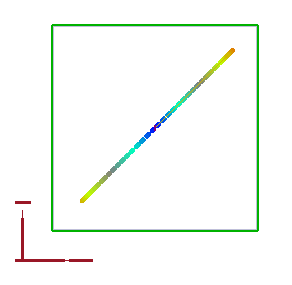
\includegraphics[width=0.475\linewidth]{graphics/Task4-lin}
		\label{fig:lin}
	}
	\subfigure[$A = 1,\: \phi_\Delta = \SI{-90}{\degree}$]
	{
		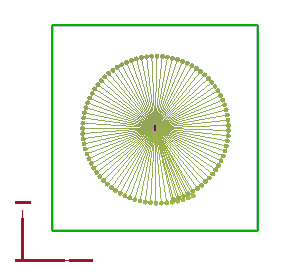
\includegraphics[width=0.475\linewidth]{graphics/Task4-RHC}
		\label{fig:RHC}
	}
	\subfigure[$A = 1,\: \phi_\Delta = \SI{45}{\degree}$]
	{
		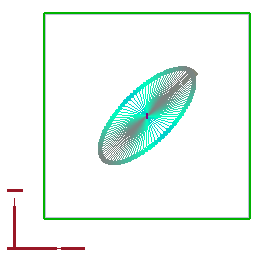
\includegraphics[width=0.475\linewidth]{graphics/Task4-LHE}
		\label{fig:LHE}
	}
	\caption{Various polarizations of a propagating electric field}
	\label{fig:polarization}
\end{figure}

Fig. \ref{fig:polarization} shows the result of changing $E_x$ and $E_y$. 

\section{Conclusion}\label{sec:conclusion}
The simulations in the lab vividly showed the electromagnetic theory that governs plane wave transmissions and reflections in a material at normal incidence.
It demonstrated how the waves behave in the first and second medium, especially the interactions of the incident wave and the reflected wave in the first medium. 

The simulation software can be used to check the calculations to see if the simulation and the calculation match up.
The reflection and transmission problems can be calculated using Smith charts. 

Electromagnetic transformers can be designed using the material properties and using materials with specific permittivity and adjusting the length of material sections to allow a specific amount of transmission. 


\newpage
\printbibliography[heading=bibintoc,title={References}]

\end{document}
